
\documentclass[a4paper]{article}
\usepackage[margin=1in]{geometry}
\usepackage[english]{babel}
\usepackage[utf8]{inputenc}
\usepackage{amsmath,amsthm,amssymb}
\usepackage{graphicx}
\usepackage{epstopdf}
\usepackage{pdfpages}
\usepackage{float, algorithmic, algorithm2e, program}
\usepackage{tabularx}
\usepackage{longtable}
\newtheorem{theorem}{Theorem}
\newtheorem{definition}{Definition}[section]

\title{Bathtub Qualitative Reasoning}
\author{Nicola De Cao, Luca Falorsi, Govert Verkes}
\date{\today}

\begin{document}
\maketitle

\section{Problem}

\begin{itemize}
\item \textbf{Quantities:}
\begin{itemize}
\item Inflow (of water into the container) $\in [0, +]$
\item Outflow (of water out of the container) $\in [0, +, Max]$
\item Volume (of the water in the container) $\in [0, +, Max]$
\end{itemize}

\item \textbf{Dependencies:}

\begin{itemize}
\item I+(Inflow, Volume): the amount of inflow increases the volume
\item I-(Outflow, Volume): the amount of outflow decreases the volume
\item P+(Volume, Outflow): outflow changes are proportional to volume changes
\item V(Volume(Max), Outflow(Max)): the outflow is at its highest value (Max), when the volume is at it highest value
\item V(Volume(0), Outflow(0)): there is no outflow, when there is no volume
\end{itemize}
\end{itemize}


\begin{figure}[H]
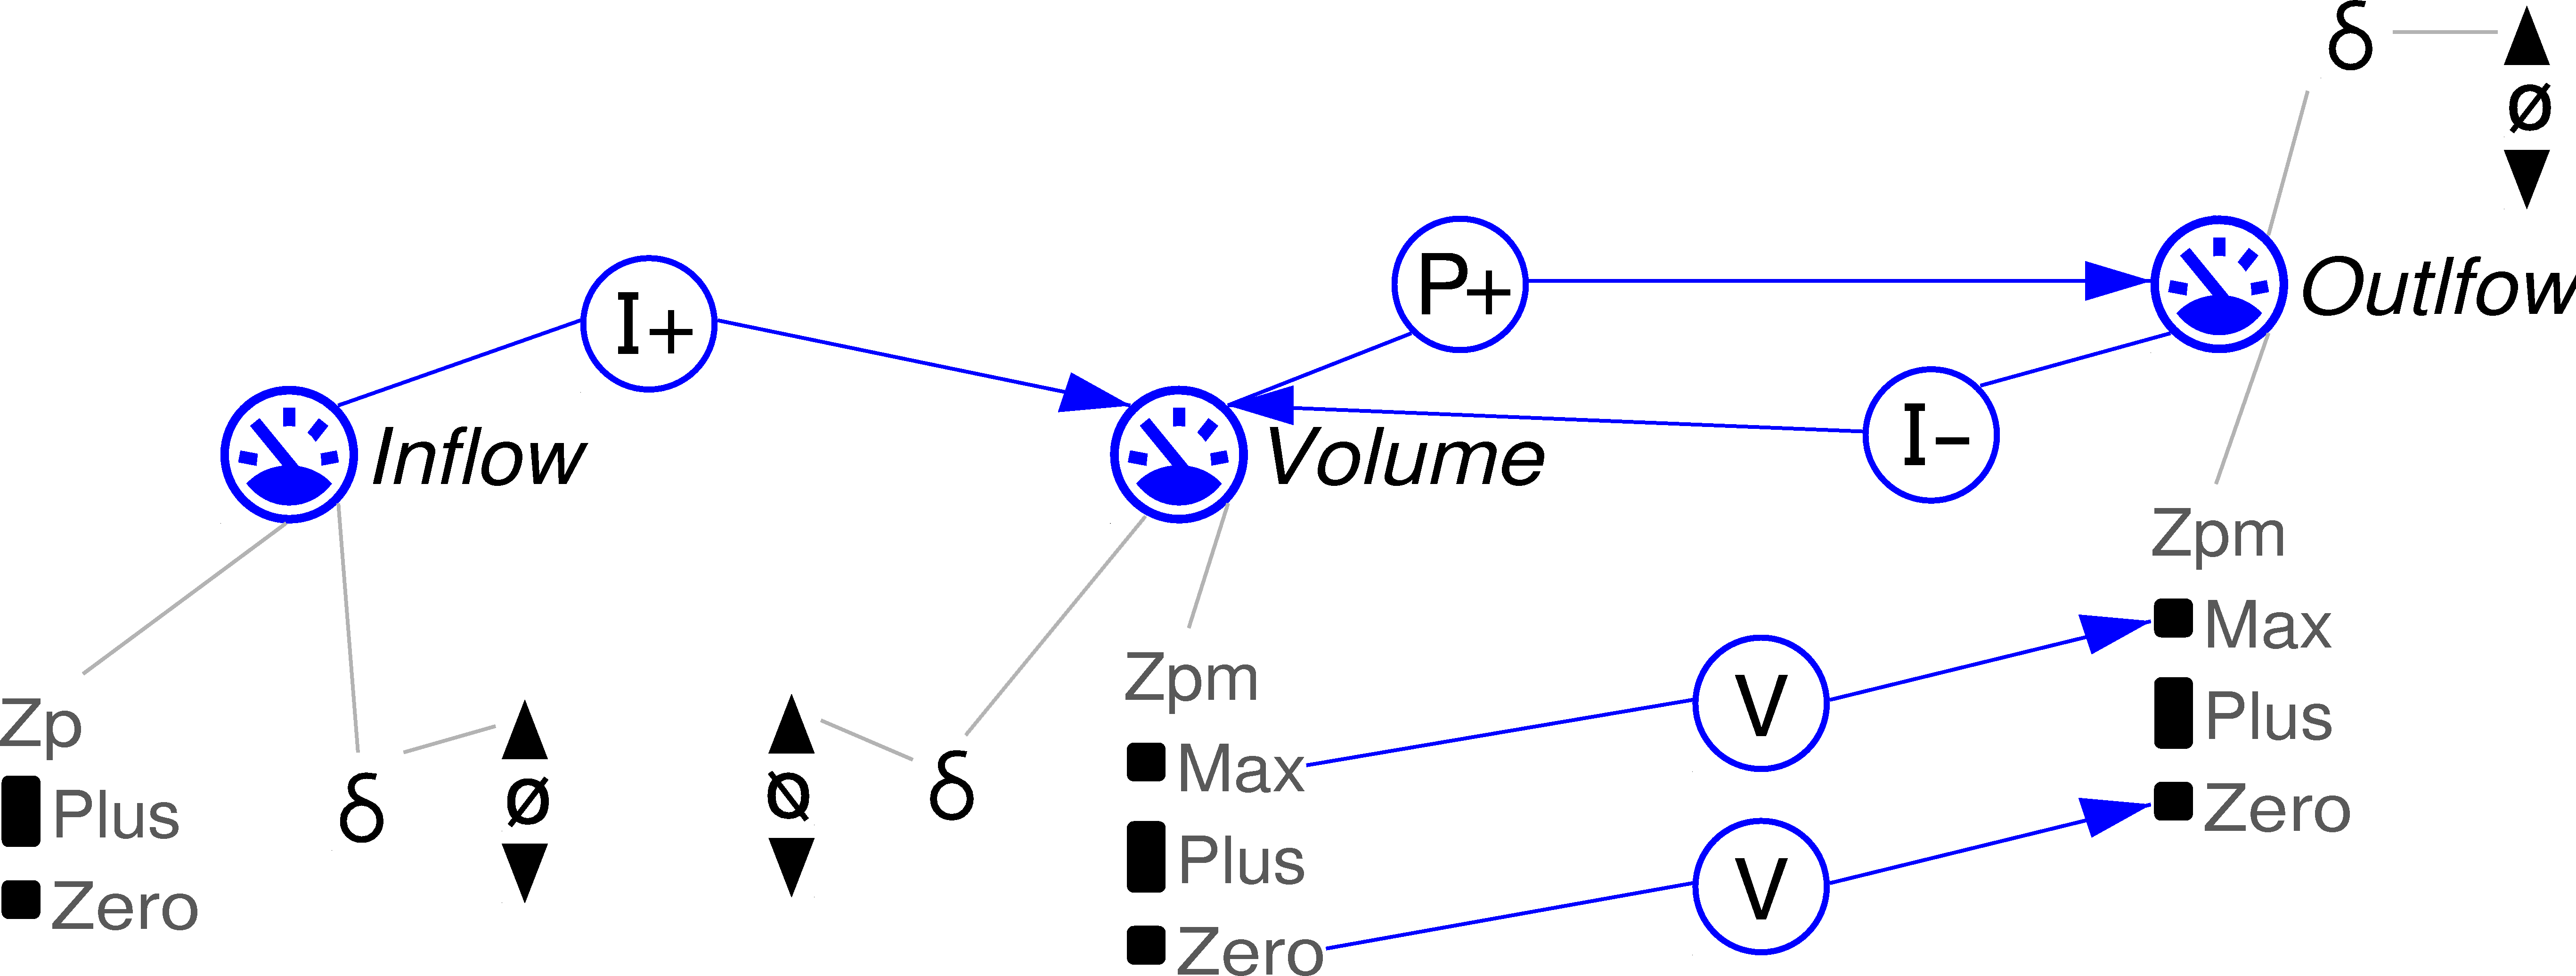
\includegraphics[]{problem.png}
\caption{Drawings of the causal model active for the system}
\end{figure}

\begin{algorithm}
\If{condition}{then-block}
\caption{Drawings of the causal model active for the system}
\end{algorithm}

\end{document}

